% F1R3FLY.IO -- Bulk import and export for the F1R3Node shard
% Design document. Build with:  latexmk -xelatex bulk-import-export.tex
% Brand system: f1r3fly-brand-kit v1.2 (2026-09-20) from F1R3FLY-io/f1r3fly-brand-portal.
% Fonts (fonts/) and logos (logos/) are copied unmodified from the brand portal.

\documentclass[10pt]{article}

% ---------------------------------------------------------------- page & grid
% A4 landscape; 6-column brand grid: 8.3% side margins, 2% gutters.
\usepackage[a4paper,landscape,
  left=24.65mm,right=24.65mm,top=20mm,bottom=24mm,footskip=12mm]{geometry}
\usepackage{multicol}
\setlength{\columnsep}{17.82mm}   % one grid column + gutters: 3+3 split
\setlength{\columnseprule}{0pt}
\raggedcolumns

% ---------------------------------------------------------------- colour
\usepackage[table]{xcolor}
\definecolor{brandblack}{HTML}{000000}
\definecolor{brandwhite}{HTML}{FFFFFF}
\definecolor{brandyellow}{HTML}{F3D630}
\definecolor{brandsky}{HTML}{3FA9F5}
\definecolor{mutedtext}{HTML}{C5C5C5}   % AAA on black
\definecolor{rulegray}{HTML}{959595}    % AA on black
\definecolor{panelline}{HTML}{3F3F3F}   % neutral gray, structure only
\pagecolor{brandblack}
\color{brandwhite}

% ---------------------------------------------------------------- type
\usepackage{fontspec}
\setmainfont{SourceSans3}[
  Path=fonts/, Extension=.ttf,
  UprightFont=*-400, BoldFont=*-700,
  ItalicFont=*-400, ItalicFeatures={FakeSlant=0.18},
  BoldItalicFont=*-700, BoldItalicFeatures={FakeSlant=0.18}]
\newfontfamily\spartan{LeagueSpartan}[
  Path=fonts/, Extension=.ttf,
  UprightFont=*-Regular, BoldFont=*-Bold]
\newfontfamily\spartanlight{LeagueSpartan-Light}[Path=fonts/, Extension=.ttf]
\newfontfamily\spartansemi{LeagueSpartan-SemiBold}[Path=fonts/, Extension=.ttf]
\newfontfamily\spartancaps{LeagueSpartan-Bold}[Path=fonts/, Extension=.ttf, LetterSpace=12]
\newfontfamily\spartansemicaps{LeagueSpartan-SemiBold}[Path=fonts/, Extension=.ttf, LetterSpace=12]
\newfontfamily\spartanlightcaps{LeagueSpartan-Light}[Path=fonts/, Extension=.ttf, LetterSpace=8]
% Monospace for manifests only. The brand system has no monospace face;
% DejaVu Sans Mono is used for code and flagged as such in the colophon.
\setmonofont{DejaVu Sans Mono}[Scale=0.84]

\linespread{1.14}
\setlength{\parindent}{0pt}
\setlength{\parskip}{0.45\baselineskip}
\usepackage{microtype}
\widowpenalty=10000 \clubpenalty=10000 \brokenpenalty=10000

% ---------------------------------------------------------------- misc
\usepackage{graphicx}
\usepackage{tikz}
\usetikzlibrary{positioning,arrows.meta,calc}
\usepackage{array,booktabs,tabularx}
\usepackage{enumitem}
\usepackage{fancyvrb}
\usepackage{fancyhdr}
\usepackage{titlesec}
\usepackage{etoolbox}
\usepackage{xurl}
\usepackage[hidelinks]{hyperref}
\hypersetup{colorlinks=true,linkcolor=brandsky,urlcolor=brandsky,
  pdftitle={Bulk Import and Export for the F1R3Node Shard},
  pdfauthor={F1R3FLY.IO}}

% gradient accent rule, 0.5pt, yellow -> sky (two stops only)
\newcommand{\gradrule}[1][\linewidth]{%
  \noindent\begin{tikzpicture}
    \shade[left color=brandyellow,right color=brandsky]
      (0,0) rectangle (#1,0.5pt);
  \end{tikzpicture}}

% tables
\arrayrulecolor{rulegray}
\setlength{\heavyrulewidth}{0.5pt}
\setlength{\lightrulewidth}{0.3pt}
\renewcommand{\arraystretch}{1.35}
\newcommand{\colhead}[1]{{\spartan\color{mutedtext}#1}}   % column headers: lowercase

% lists
\setlist{leftmargin=1.1em,itemsep=0.35\baselineskip,topsep=0.2\baselineskip,parsep=0pt}
\setlist[itemize]{label={\color{brandsky}\textbullet}}
\setlist[enumerate]{label={\color{brandyellow}\spartan\arabic*}}

% ---------------------------------------------------------------- headings
% Part = page title: ALL-CAPS, letter-spaced, top of a new page, gradient under it.
\newcommand{\pagetitle}[2][]{%
  \clearpage
  \phantomsection\addcontentsline{toc}{section}{#2}%
  \vspace*{2mm}%
  {\fontsize{26}{30}\selectfont\spartancaps\MakeUppercase{#2}\par}%
  \vspace{5mm}\gradrule\par
  \ifstrempty{#1}{}{\vspace{4mm}{\color{mutedtext}#1}\par}%
  \vspace{7mm}}
% Section = subheader: League Spartan SemiBold, caps, Brand Yellow, body size.
\titleformat{\section}{\spartansemicaps\color{brandyellow}}{\thesection\hspace{0.9em}}{0pt}{\MakeUppercase}
\titlespacing*{\section}{0pt}{1.4\baselineskip}{0.6\baselineskip}
% Subsection = sentence case, white, League Spartan SemiBold, body size.
\titleformat{\subsection}{\spartansemi\color{brandwhite}}{}{0pt}{}
\titlespacing*{\subsection}{0pt}{1.0\baselineskip}{0.25\baselineskip}
\setcounter{secnumdepth}{1}

% panel for manifests and callouts
\newenvironment{panel}{%
  \par\smallskip\noindent
  
\begin{tikzpicture}\node[draw=panelline,line width=0.5pt,rounded corners=4pt,
    inner sep=3.2mm,text width=\dimexpr\linewidth-6.4mm-1pt\relax,align=left]\bgroup}%
  {\egroup;\end{tikzpicture}\par\smallskip}

\DefineVerbatimEnvironment{manifest}{Verbatim}{formatcom=\color{mutedtext},
  baselinestretch=1.05,frame=leftline,framerule=0.5pt,rulecolor=\color{brandsky},
  framesep=3.5mm,xleftmargin=0.5mm}

% ---------------------------------------------------------------- footer
\pagestyle{fancy}
\fancyhf{}
\renewcommand{\headrulewidth}{0pt}
\fancyfoot[L]{\raisebox{-1.2mm}{
\includegraphics[height=5mm]{logos/f1r3fly-io-bug-icon-color-on-dark.pdf}}%
  \hspace{3mm}{\fontsize{7}{9}\selectfont\spartancaps\color{mutedtext}\thepage}}
\fancyfoot[R]{\fontsize{7}{9}\selectfont\spartancaps\color{mutedtext}%
  © F1R3FLY.IO, 2026. ALL RIGHTS RESERVED \textbar\ OCTOBER 10, 2026}

\begin{document}

% ================================================================= COVER
\thispagestyle{empty}
\begin{tikzpicture}[remember picture,overlay]
  \coordinate (O) at ($(current page.north west)+(24.65mm,-26mm)$);
  \node[anchor=north west,inner sep=0] at (O)
    {
\includegraphics[height=40mm]{logos/f1r3fly-io-vertical-logo-color-on-dark.pdf}};
  \node[anchor=north west,inner sep=0,text=brandyellow] at ($(O)+(0,-66mm)$)
    {\spartancaps DESIGN DOCUMENT \textbar\ DRAFT FOR INTERNAL REVIEW};
  \node[anchor=north west,inner sep=0,text=brandwhite,align=left] at ($(O)+(0,-76mm)$)
    {\fontsize{34}{40}\selectfont\spartanlight Bulk import and export\\[1mm]
     \fontsize{34}{40}\selectfont\spartanlight for the F1R3Node shard};
  \shade[left color=brandyellow,right color=brandsky]
    ($(O)+(0,-108mm)$) rectangle ++(160mm,0.5pt);
  \node[anchor=north west,inner sep=0,text=mutedtext,text width=125mm,align=left]
    at ($(O)+(0,-118mm)$)
    {A general shard capability for moving large external datasets into and out
     of a F1R3FLY shard as committed, verifiable, capability-secured state.
     OpenStreetMap is the motivating case; the mechanism is not specific to it.};
  \node[anchor=north west,inner sep=0,text=brandwhite,align=left]
    at ($(O)+(165mm,-118mm)$)
    {{\spartan\color{mutedtext}author}\\ Lucius Gregory Meredith\\[2mm]
     {\spartan\color{mutedtext}date}\\ October 10, 2026\\[2mm]
     {\spartan\color{mutedtext}status}\\ Draft, version 0.1};
\end{tikzpicture}
\null

% ================================================================= OVERVIEW
\pagetitle[What the capability is, why it is needed, and where data can land.]{Overview}

\begin{multicols}{2}

\section{Summary}

This note specifies a generic bulk importer and a matching exporter for the
F1R3Node shard. The importer lets a dataset of any size enter the shard as
committed state that every validator agrees on, without routing billions of
records through individual deploys and without a side door that sits outside
consensus.

The core is a two-phase \emph{bulk update}: a \textbf{stage} deploy names a
content-addressed source and a pinned transformer; validators fetch and
transform out of band and attest the root they computed; a cheap \textbf{commit}
deploy swaps that root in once a quorum agrees. Genesis loading becomes one use
of this mechanism rather than a special case.

Around that core sits an import manifest that declares where each field lands
(channels, consensus-mode files or oracular files), how records are laid out and
indexed, which capabilities and guards the new namespace is born with, and how
later deltas arrive. The exporter is the same contract run in reverse.

The scope test for every feature is simple. The importer does only what must
happen at the moment data enters, deterministically, inside the staged step.
Anything that can be done afterwards by a rholang program over the imported data
is out of scope.

\section{Motivation}

\subsection{Data should roll in}

A standing business aim of F1R3FLY.IO is to tilt the field so that data moves
into the shard because of what it gains there: guarded where-clauses over access,
agentic coordination over who may use what, object-capability security, and
verifiable provenance. That aim fails at the first step if getting a large
existing dataset in is expensive, slow or unsafe. A first-class bulk path is the
on-ramp for every web 2 backend replacement studied in Spring 2026 and for any
customer bringing an existing corpus.

\subsection{The OpenStreetMap case}

OpenStreetMap keeps its authoritative data in a single PostgreSQL cluster behind
the Rails port and CGImap, with current and history tables for nodes, ways and
relations, plus changesets, users and GPX traces. In March 2026 the database held
about 11.7 billion objects: 10.5 billion nodes (only 2.7\% of them tagged),
1.17 billion ways and 14.2 million relations. The data is not large blobs; it is
an enormous number of tiny records.

\subsection{Two options that were rejected}

\textbf{A sidecar store beside each node.} Keeping the existing database next to
every validator, with all access forced through the node, does not give
replication for free. External state is not covered by the block state hash, so
copies can drift without detection. Rholang execution is speculative, so the
store would need rollback to an arbitrary block, and sequence-generated keys leave
gaps on rollback that break determinism. A joining validator would need a
snapshot matching an exact block. Making all of that sound amounts to rebuilding
state-machine replication inside the database, and every operation would pay for
inter-process communication.

\textbf{Ordinary deploys, or genesis only.} Pushing billions of elements through
deploys is far too slow. Loading at genesis works once but rules out every later
import into a running shard. Both limitations disappear if a bulk update is a
proper consensus operation.

\section{Where data can land}

The node offers three storage surfaces. File IO is now implemented and merged on
the \texttt{dev} branch of f1r3node-rust, so large data no longer has to pass
through LMDB as it does in F1R3Drive today.

\vspace{2mm}
\begin{tabularx}{\linewidth}{@{}>{\spartansemi}p{0.27\linewidth}X@{}}
\toprule
\colhead{surface} & \colhead{properties and typical use} \\
\midrule
RSpace channels &
  Fine-grained, guarded, reactive; every datum is a process-level object. Best
  for indices, small hot records and anything contracts react to. \\
Files, \texttt{consensus} mode &
  Mutations journaled to the consensus write-ahead log, re-executed and verified
  by every validator. Best for the bulk of authoritative data, laid out in chunk
  files whose hashes live in RSpace. \\
Files, \texttt{oracular} mode &
  Not replicated; reachable only through the validator connected to the external
  service or data. Best for personal, licensed or unpublishable fields. \\
\bottomrule
\end{tabularx}
\vspace{2mm}

A single import may route different fields of the same record to different
surfaces. That routing is part of the manifest (Section~\ref{sec:manifest}).

\end{multicols}

% ================================================================= FIT WITH NODE
\pagetitle[What file IO on the dev branch already provides, and what that means for this design.]{Fit with node file IO}

\begin{multicols}{2}

\section{What the node already provides}

This section reflects the \texttt{dev} branch of f1r3node-rust at commit
\texttt{93e3282} (October 10, 2026).

\subsection{Modes per bundle entry}
Each filesystem bundle entry carries a mode, \texttt{consensus} or
\texttt{oracular}. In consensus mode, host-transient metadata (modification,
change and access times, owner, group) is omitted from \texttt{stat} and directory
listings, and \texttt{chown} is refused. Part of the determinism discipline the
importer needs is therefore already enforced at the surface.

\subsection{Replication by write-ahead log}
Every consensus-mode mutation is recorded as a write-ahead-log entry. Entries
carry a Blake2b-256 hash of the payload, not the bytes. Followers re-execute the
same operation against their own filesystem and compare the hash of their reply
with the leader's, and the WAL root is committed per block. Oracular entries are
not replicated.

\subsection{Snapshots and joining validators}
Snapshots are log-structured: canonical encodings of WAL slices, not images of
filesystem state. Each is split into 4 MiB chunks under a domain-separated binary
Merkle tree, and the root is committed on-chain. A joining validator fetches and
verifies chunks from peers, then fetches referenced payloads by hash. The
joiner-side payload sync is partly landed.

\subsection{Provisioning}
Consensus roots are provisioned per bundle at genesis or boot. The native
filesystem URNs resolve only in genesis deploys; user deploys reach files through
the published Fs capability.

\subsection{Hard caps}
\vspace{1mm}
\begin{tabularx}{\linewidth}{@{}>{\spartansemi}p{0.47\linewidth}X@{}}
\toprule
\colhead{cap} & \colhead{value} \\
\midrule
Bytes per read or write & 64 MiB \\
File length (truncate ceiling) & 16 GiB \\
Entries per directory listing & 65,536 \\
WAL entries per runtime & 65,536 \\
Open file descriptors & 1,024 \\
\bottomrule
\end{tabularx}

Every one of these is a fingerprinted consensus constant; changing any of them is
a coordinated network upgrade.

\section{Consequences for this design}

\subsection{The commit is one new WAL operation}
The protocol's attest step is the same discipline the node already uses,
re-execute and compare hashes, moved outside the block so it can take hours. The
commit then appends a single bulk-apply entry to the consensus WAL, whose payload
reference is the staged result root. The WAL operation set is part of the
consensus fingerprint, so adding this operation ships as a coordinated network
upgrade.

\subsection{Reuse the existing hash and chunk construction}
Source roots and result roots use Blake2b-256 and the same 4 MiB chunk Merkle tree
as WAL snapshots. The staging fetch reuses the snapshot chunk retriever and
payload sync rather than inventing a second transfer protocol.

\subsection{Joiners must not rerun the transform}
Because snapshots are log-structured replay from genesis, a joining validator
would otherwise replay every bulk commit. The bulk-apply entry must reference the
content-addressed result tree so a joiner fetches output chunks by hash. A single
planet-sized commit also argues for materialized checkpoints of bulk namespaces;
see Section~\ref{sec:open}.

\subsection{The caps shape the layout}
A directory listing returns at most 65,536 entries, so partitioned data needs a
hierarchy of prefix directories. A geohash layout, for example, nests cells under
two-character prefix directories. Each chunk file should stay well under the
64 MiB read cap so ordinary contracts can read a whole cell in one call.

\subsection{Deploy-based import is ruled out by the caps}
With at most 65,536 WAL entries per runtime, and every payload carried in deploy
data, an import through ordinary deploys would take many thousands of deploys even
at file granularity. This confirms the case for a dedicated bulk path.

\subsection{Targets must be provisioned roots}
A bulk update can only land in a provisioned consensus root. Importing into a new
namespace on a running shard needs either an import root provisioned in advance,
under which namespaces are created as subdirectories, or runtime extension of the
bundle. This is an open question.

\end{multicols}

% ================================================================= PROTOCOL
\pagetitle[The two-phase bulk update that every import and delta uses.]{The bulk update protocol}

\begin{center}
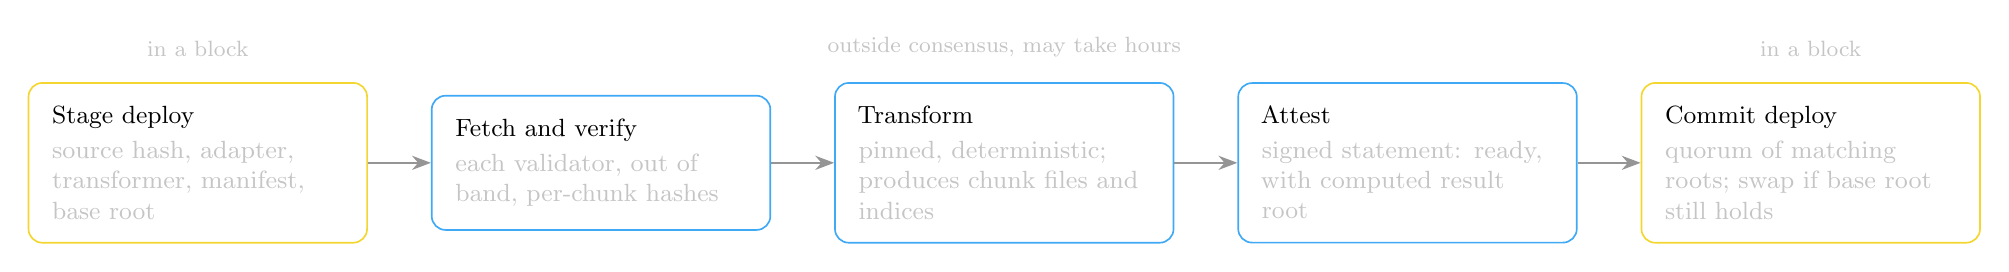
\begin{tikzpicture}[
  font=\small,
  box/.style={draw=brandsky,line width=0.6pt,rounded corners=5pt,
    minimum height=17mm,text width=37mm,align=left,inner sep=3mm},
  chain/.style={draw=brandyellow,line width=0.6pt,rounded corners=5pt,
    minimum height=17mm,text width=37mm,align=left,inner sep=3mm},
  arr/.style={-{Stealth[length=2.4mm]},line width=0.6pt,color=rulegray},
  lab/.style={font=\spartan\footnotesize,color=mutedtext}]
  \node[chain] (stage) {{\spartansemi Stage deploy}\\[0.5mm]{\color{mutedtext}source hash, adapter, transformer, manifest, base root}};
  \node[box,right=8mm of stage] (fetch) {{\spartansemi Fetch and verify}\\[0.5mm]{\color{mutedtext}each validator, out of band, per-chunk hashes}};
  \node[box,right=8mm of fetch] (xform) {{\spartansemi Transform}\\[0.5mm]{\color{mutedtext}pinned, deterministic; produces chunk files and indices}};
  \node[box,right=8mm of xform] (attest) {{\spartansemi Attest}\\[0.5mm]{\color{mutedtext}signed statement: ready, with computed result root}};
  \node[chain,right=8mm of attest] (commit) {{\spartansemi Commit deploy}\\[0.5mm]{\color{mutedtext}quorum of matching roots; swap if base root still holds}};
  \draw[arr] (stage) -- (fetch);
  \draw[arr] (fetch) -- (xform);
  \draw[arr] (xform) -- (attest);
  \draw[arr] (attest) -- (commit);
  \node[lab,above=2mm of stage] {in a block};
  \node[lab,above=2mm of commit] {in a block};
  \node[lab,above=2mm of xform] {outside consensus, may take hours};
\end{tikzpicture}
\end{center}
\vspace{4mm}

\begin{multicols}{2}

\section{Why two phases}

A planet-scale fetch and transform takes hours, far beyond any block's execution
budget. If it ran inside a block, one validator that could not reach the source
would be unable to validate the block and the shard would stall. Splitting the
work keeps both consensus steps cheap and puts the slow, failure-prone part where
it can be retried without holding up anything else.

\section{The stage deploy}

The stage deploy records an intent. It carries:

\begin{itemize}
\item \textbf{Source locations and content hash.} The hash is a Blake2b-256 Merkle
  root over 4 MiB source chunks, built exactly as for WAL snapshots. Validators fetch from any listed location,
  mirror or peer and verify against the hash, so the source needs to be available
  but not trusted.
\item \textbf{Adapter and transformer hashes.} The adapter reads the source format;
  the transformer maps records to target layout. Both are pinned by hash, so every
  validator runs exactly the same code.
\item \textbf{Manifest hash.} The declarative description of mapping, layout,
  indices, capabilities and validation (Section~\ref{sec:manifest}).
\item \textbf{Base root.} The state root of the target namespace that the update
  applies to. For a first import this is the empty namespace.
\item \textbf{Expected result root (optional).} When the publisher has computed it,
  it lets validators detect a disagreement immediately rather than at commit.
\item \textbf{Capability and payment.} The bulk-update capability for the target
  namespace, and the deposit covering the operation (Section~\ref{sec:cost}).
\item \textbf{Expiry.} A height after which an uncommitted stage lapses.
\end{itemize}

\section{Validator work and attestation}

On seeing a stage in a finalized block, each validator fetches the chunks it
lacks, verifies them against the source root, runs the adapter and transformer,
and writes the output into a staging area of consensus-mode files that is not yet
visible to contracts. It then submits a signed attestation: the stage identifier
and the result root it computed, covering the chunk files, their RSpace index
entries and the reject log.

Chunk-level hashing makes the work resumable after a failure and lets validators
exchange verified source chunks with each other, which spreads the load off the
original source.

\section{The commit deploy}

The commit deploy references the stage and is valid only if a quorum of bonded
validators has attested the same result root and the target namespace is still at
the base root. Execution is a root swap: the staged files become the namespace's
committed content and the index entries become visible. The commit costs about
as much as any small deploy. In the node, the swap is a single bulk-apply entry
in the consensus WAL whose payload reference is the result root.

A validator that had not finished its own transform when the commit lands syncs
the committed chunks from peers by hash and verifies them against the committed
root, using the same payload sync a late-joining validator uses.

\section{Determinism requirements}

The protocol is only sound if the transform is a pure function of the source
bytes, the adapter, the transformer and the manifest. Concretely:

\begin{itemize}
\item no reads of time, locale, environment, randomness or network inside the
  transform (consensus mode already strips host-transient file metadata);
\item a canonical output encoding, with records sorted by a declared key and
  chunk boundaries fixed by rule rather than by buffer sizes;
\item no floating-point results that depend on platform or instruction order;
  coordinates and other reals are stored in the source's fixed-point form or a
  declared canonical decimal;
\item the reject log is part of the output and is itself canonical.
\end{itemize}

The open question of which language transformers are written in (rholang or
f1r3lang, or a sandboxed WASM module) is listed in Section~\ref{sec:open}.

\section{Failure modes}

\vspace{1mm}
\begin{tabularx}{\linewidth}{@{}>{\spartansemi}p{0.3\linewidth}X@{}}
\toprule
\colhead{failure} & \colhead{outcome} \\
\midrule
Attested roots disagree &
  No commit. The disagreement is evidence of a faulty validator or a
  non-deterministic transformer, and is recorded as such. \\
Source unreachable &
  Validators cannot attest. The stage lapses at expiry; the deposit covers the
  work already done. \\
Namespace changed since staging &
  The base-root check fails at commit. The publisher restages against the new
  root, as a delta if the change is small. \\
Validator slow or offline &
  Commit proceeds on quorum; the validator syncs committed chunks from peers. \\
\bottomrule
\end{tabularx}

\end{multicols}

% ================================================================= MANIFEST
\pagetitle[The declarative description that accompanies every stage.]{The import manifest}

\begin{multicols}{2}

\section{Shape}\label{sec:manifest}

The manifest is what makes the importer generic. It is data, hashed into the
stage deploy, and it says everything the transformer needs beyond the source
bytes. The example below is illustrative; the concrete syntax is not yet fixed.

\begin{manifest}
[source]
format    = "osm-pbf"
adapter   = "blake2b256:9c1e...a07b"
root      = "blake2b256:41d2...e9f0"
watermark = { kind = "replication-seq",
              value = 6_214_377 }

[target]
root      = "import"        # provisioned
namespace = "osm/planet"
cap       = "ocap:osm-import"

[layout.nodes]
surface   = "consensus-file"
partition = "geohash(lat, lon, 5)"
path      = "{gh[0:2]}/{gh[2:4]}/{gh}"
encoding  = "canonical-cbor"
sort_key  = ["id"]

[layout.users]
surface   = "oracular-file"
redact    = ["email", "pass_crypt"]

[[index]]
on   = "nodes"
key  = "id"
kind = "point"

[[index]]
on   = "ways"
key  = "node_refs[]"
kind = "reverse"

[access]
owner = "ocap:osm-foundation"
read  = "public"
write = "guard:changeset-open"

[validation]
schema  = "osm-0.6"
on_fail = "reject-and-log"

[delta]
stream = "osmchange-minutely"
\end{manifest}

\section{Schema mapping}

Generic schema-mapping support is deliberately modest. It covers what is needed
to place records, not to improve them:

\begin{itemize}
\item field selection, renaming and type coercion to canonical types;
\item nesting and flattening between the source shape and the target shape;
\item key derivation: how the namespace name of a record or chunk is built from
  its key fields;
\item per-field routing to a surface, which is how one record can keep its public
  fields in consensus files and its private fields in oracular storage;
\item computed partition keys, such as a geohash cell, supplied as pinned
  transformer functions rather than as built-in features.
\end{itemize}

Cleaning, deduplication, entity resolution and enrichment are not mapping. They
belong in rholang programs over imported data.

\section{Features}

\subsection{1. Provenance as committed state}
Each import records the source root, the adapter, transformer and manifest
hashes, the source watermark, the authorizing capability and the block of the
commit. Every imported item can be traced back to its import event. Imported data
gains a verifiable lineage it did not have at the source.

\subsection{2. Capabilities assigned at birth}
The manifest declares the namespace owner, read and write capabilities, and any
guards. Default is deny. Imported data never exists unsecured, even for one block,
and the access channels that agents use to negotiate access are present from the
first commit.

\subsection{3. Three targets, with redaction before staging}
Staged files replicate, so redaction must happen in the transform, not afterwards.
Personal data, licensed fields and anything the owner will not publish to every
validator are routed to oracular storage or dropped at mapping time.

\subsection{4. Layout and declared indices}
The manifest fixes granularity: one record per channel, or records chunked into
files by a partition key. It also declares the indices to build. Building indices
later would mean a second full pass, and they must be built deterministically
along with the data. Declared key, range and reverse indices are built in; spatial,
full-text and other specialized indices plug in as hashed transformers.

\subsection{5. Snapshot plus deltas}
An initial load and its change streams (osmChange files, PostgreSQL logical
replication, CDC feeds) are all bulk updates conditioned on a base root. A replayed
delta fails the base-root check, so replay is harmless. Without deltas, ``rolling
in'' stops at a one-time migration.

\subsection{6. Deterministic validation and a reject log}
Records that fail the declared schema are rejected, not repaired. The reject log,
with the reason for each rejection, is committed with the data so every validator
agrees on exactly what was admitted.

\subsection{7. Chunked, Merkle-structured staging}
Per-chunk hashes make fetching resumable, let validators share verified chunks,
and let a lagging validator catch up from peers.

\subsection{8. Dry run and cost quote}
Before staging, a dry run reports output size, record counts, rejects and the
cost quote. Nobody should discover the price of a planet import by performing one.

\subsection{9. Reconciliation and rollback}
After commit, a reconciliation report gives counts and checksums against the
source. Since a commit is a root swap, it can be reverted to the base root until
other writes build on it.

\subsection{10. A narrow adapter interface}
An adapter turns a source format (CSV, Parquet, JSON Lines, PBF, an SQL dump) into
a stream of records. Adapters are pinned by hash like transformers. All format
diversity lives behind this one interface.

\end{multicols}

% ================================================================= EXPORT, COST, SCOPE
\pagetitle[The way back out, who may run a bulk update, what it costs, and what is left out.]{Export, policy and scope}

\begin{multicols}{2}

\section{The exporter}

Owners are more willing to bring data in when they can see the way back out, so
the exporter is part of the on-ramp, not a concession. It is a separate tool that
shares the importer's manifest model and adapters, run in reverse.

\begin{itemize}
\item \textbf{Snapshot export.} Any node can produce a snapshot of a namespace as
  of a given block, in any format with a writer adapter, together with the block
  hash and namespace root, so the consumer can verify it without trusting the
  exporting node.
\item \textbf{Change-feed export.} Committed blocks touching a namespace are
  emitted as a delta stream in the consumer's format, carrying the same proofs.
\item \textbf{Capabilities apply.} Export requires the read capability. Oracular
  fields are exported only through the validator connected to their source.
\item \textbf{Receipts are optional.} Export does not change state and needs no
  consensus. An owner who wants accountability over exports can require a small
  receipt deploy recording who exported what, as of which block.
\end{itemize}

\section{Access and cost}\label{sec:cost}

\subsection{Access}
The bulk-update capability is distinct from ordinary write access and is gated by
object capabilities on the target namespace. Without the gate, a stage deploy
would be a cheap way to make every validator download and process terabytes.

\subsection{Cost}
The ordinary per-operation cost model does not price this operation, so it needs
its own rule. The working proposal is a deposit at staging, proportional to the
quoted output size and chunk count, that compensates validators for fetch,
transform and storage; a small fee at commit; and forfeiture of part of the deposit
if the stage lapses. Storage rent for the committed data then follows whatever
rule the shard applies to consensus-mode files.

\section{Out of scope}

These are rholang programs over imported data, or separate tools:

\begin{itemize}
\item cleaning, deduplication and entity resolution;
\item enrichment, and joins across sources;
\item scheduling and orchestration of recurring pipelines;
\item query and analytics.
\end{itemize}

The line is drawn where determinism and the moment of entry stop mattering.
Everything inside the line must be identical on every validator and must happen
before data is visible; everything outside it can run later, as ordinary
computation, under the same capabilities as any other program.

\section{Generality}

Nothing in the protocol is specific to maps. The same mechanism serves the other
Spring 2026 properties, such as bulk loading document blobs for the OnlyOffice
backend, and any customer corpus. Genesis loading is a stage and commit against
an empty shard.

\end{multicols}

% ================================================================= OSM
\pagetitle[How OpenStreetMap would use the capability, and what it changes in the Spring plan.]{Worked example: OpenStreetMap}

\begin{multicols}{2}

\section{Initial load}

\begin{enumerate}
\item The publisher takes a planet PBF at a known replication sequence number and
  publishes it with its chunk Merkle root.
\item A dry run reports output size, record counts and rejects.
\item The stage deploy names the PBF, the PBF adapter, an OSM transformer and the
  manifest shown earlier, against the empty \texttt{osm/planet} namespace.
\item Validators lay nodes, ways and relations out as consensus-mode files per
  geohash cell, in a compact canonical encoding, nested under two-character prefix
  directories to respect the directory-listing cap. RSpace holds only per-cell
  content hashes and the declared indices.
\item User records are not in the public dumps in any case. Any user data that is
  imported goes to oracular storage, with email and credential fields dropped.
\item On a quorum of matching roots, the commit swaps in the namespace.
\end{enumerate}

\section{Catch-up and cutover}

Minutely osmChange files are applied as delta stages, batched as needed, each
conditioned on the previous root. When the shard is within a few minutes of the
live database, editors are pointed at the API facade and the shard becomes
authoritative. After cutover, edits arrive as ordinary deploys; the delta path
stays available for later imports from government and other open-data sources.

\section{Why the data model changes}

The Spring plan gave each element its own channel and registered it under geohash
prefixes at three precision levels. At 11.7 billion objects that is tens of
billions of LMDB entries, and record count, not byte count, is the bottleneck.
Cell files with indexed hashes bring the record count in RSpace down by several
orders of magnitude. An edit rewrites one cell file and commits its new hash.

\section{Changes to the Spring plan}

\begin{itemize}
\item The importer moves from the migration phase (months 10--12) to the start,
  because the spatial index cannot be benchmarked meaningfully without
  planet-scale data.
\item The data model moves from one channel per element to per-cell files in
  consensus mode.
\item The bulk-update protocol is built as a shard feature, not as OSM tooling.
\item A decision is needed on full history versus current data only.
\end{itemize}

\end{multicols}

% ================================================================= OPEN + NEXT
\pagetitle[Decisions still to make and the order of work.]{Open questions and next steps}

\begin{multicols}{2}

\section{Open questions}\label{sec:open}

\begin{enumerate}
\item \textbf{Commit quorum.} What fraction of bonded stake must attest a matching
  root, and how is that tied to the shard's existing finality threshold?
\item \textbf{Transform trust.} Must every validator run the transform, or may some
  accept peer-transformed chunks? Source chunks verify by hash; transformed output
  does not, unless it is re-executed or accompanied by a proof.
\item \textbf{Transformer language.} rholang or f1r3lang, which keeps everything
  in one semantics and under cost accounting, or a sandboxed WASM module, which
  reuses existing parsers for formats like PBF and Parquet.
\item \textbf{Stage expiry and deposits.} The lapse height, and how much of the
  deposit is forfeited when a stage lapses through no fault of the publisher.
\item \textbf{Concurrency during staging.} How a namespace that receives ordinary
  writes while a large stage is in progress is rebased, and whether staging should
  lock a namespace or a region of it.
\item \textbf{Multi-shard targets.} How one stage targets several shards when data
  is partitioned geographically, and whether the commit is atomic across them.
\item \textbf{Export proofs.} The proof format a consumer checks against a block
  hash and namespace root.
\item \textbf{OSM history.} Whether to import full element history or current
  data only.
\item \textbf{Target provisioning.} Whether bulk updates land only under a
  pre-provisioned import root, with namespaces as subdirectories, or whether
  consensus roots can be added to the bundle on a running shard.
\item \textbf{Checkpoints for joiners.} Whether bulk namespaces get materialized
  checkpoints, so a joining validator fetches current cell files instead of
  replaying every bulk commit from genesis.
\item \textbf{Upgrade path.} Adding the bulk-apply WAL operation changes a
  fingerprinted consensus constant. It should be scheduled with any other pending
  WAL format change in one coordinated upgrade.
\end{enumerate}

\section{Next steps}

\begin{enumerate}
\item A protocol spike on a small dataset, such as a single-state OSM extract,
  through stage, attest and commit on a three-validator shard, built on the
  existing WAL, snapshot chunker and payload sync.
\item The manifest format, the adapter interface, and adapters for CSV, Parquet
  and PBF.
\item The dry run, cost quote and reconciliation report.
\item A planet-scale run, used also as the benchmark for the OSM spatial index.
\item Delta streams, starting with osmChange and PostgreSQL logical replication.
\item The exporter, snapshot first, then change feed.
\end{enumerate}

\section{Sources}

{\color{mutedtext}
Object counts: OpenStreetMap Taginfo, database statistics, data as of March 28,
2026. \url{https://taginfo.openstreetmap.org/reports/database_statistics}

Main database layout: OpenStreetMap Wiki, ``Database.''
\url{https://wiki.openstreetmap.org/wiki/Database}

File IO behaviour and caps: f1r3node-rust, \texttt{dev} branch at commit
\texttt{93e3282}; \nolinkurl{rholang/src/rust/interpreter/io/} and
\nolinkurl{casper/src/rust/genesis/contracts/fs_genesis.rs}.

Set in League Spartan and Source Sans 3 from the F1R3FLY brand portal (brand kit
v1.2). Manifest listings use DejaVu Sans Mono, since the brand system does not
yet define a monospace face.\par}

\end{multicols}

\end{document}
